% ===========================================
% HOMEWORK 2: Research Topic Quad Chart
% Written by: Braidan Duffy
%
% Date: 01/04/2023
% Last Revision: 01/05/2023
% ============================================

\documentclass[
	letterpaper, % Page size
	fontsize=10pt, % Base font size
	twoside=true, % Use different layouts for even and odd pages (in particular, if twoside=true, the margin column will be always on the outside)
	%open=any, % If twoside=true, uncomment this to force new chapters to start on any page, not only on right (odd) pages
	%chapterentrydots=true, % Uncomment to output dots from the chapter name to the page number in the table of contents
	numbers=noenddot, % Comment to output dots after chapter numbers; the most common values for this option are: enddot, noenddot and auto (see the KOMAScript documentation for an in-depth explanation)
]{kaobook}

\usepackage{pdfpages}
\usepackage{array}

\begin{document}

\pagelayout{wide} % Remove margin

\chapter*{Homework 2: Research Topic Quad Chart}

\section*{Overview}
For this assignment, you team will create a quad chart explaining your proposed research topic that you will explore during the semester.
Be sure to come up with a unique topic that is exciting and can sustain your group for the entire semester!

It is okay if your team does not come up with a research topic.
In that event, you will be asked to research the relationship between a surfer's motion and the wave characteristics using three unique non-dimensional parameters.

You may use the example below \underline{\textbf{\emph{as a reference}}}

\section*{Requirements}
The chart must conform to the following format:

\vspace{0.5cm}

{
\setlength\extrarowheight{4pt}
\begin{table}[h!]
	\label{tab:quad_chart format}
	\begin{tabular}{| p{0.3\linewidth} | p{0.3\linewidth} |}
		\hline
		\textbf{Introduction} \newline Introduce your team members and team name. Describe your topic and goals. & 
		\textbf{Required Sensors and Measured Variables} \newline Describe what sensors you think you would need and what data you would use from them. \\
		\hline
		\textbf{Motivations} \newline Describe your team's motivation for choosing this research topic &
		\textbf{Contributions to Society} \newline Describe how exploring the research question benefits society \\
		\hline
	\end{tabular}
\end{table}
}

\section*{Grading}
This assignment will use a pass-forgive scheme.
You must convince the instructor that your research topic is worthy using this quad chart.
If you fail to do so, or do not submit a quad chart, the grade will be forgiven and your team will be tasked with researching the default prompt.

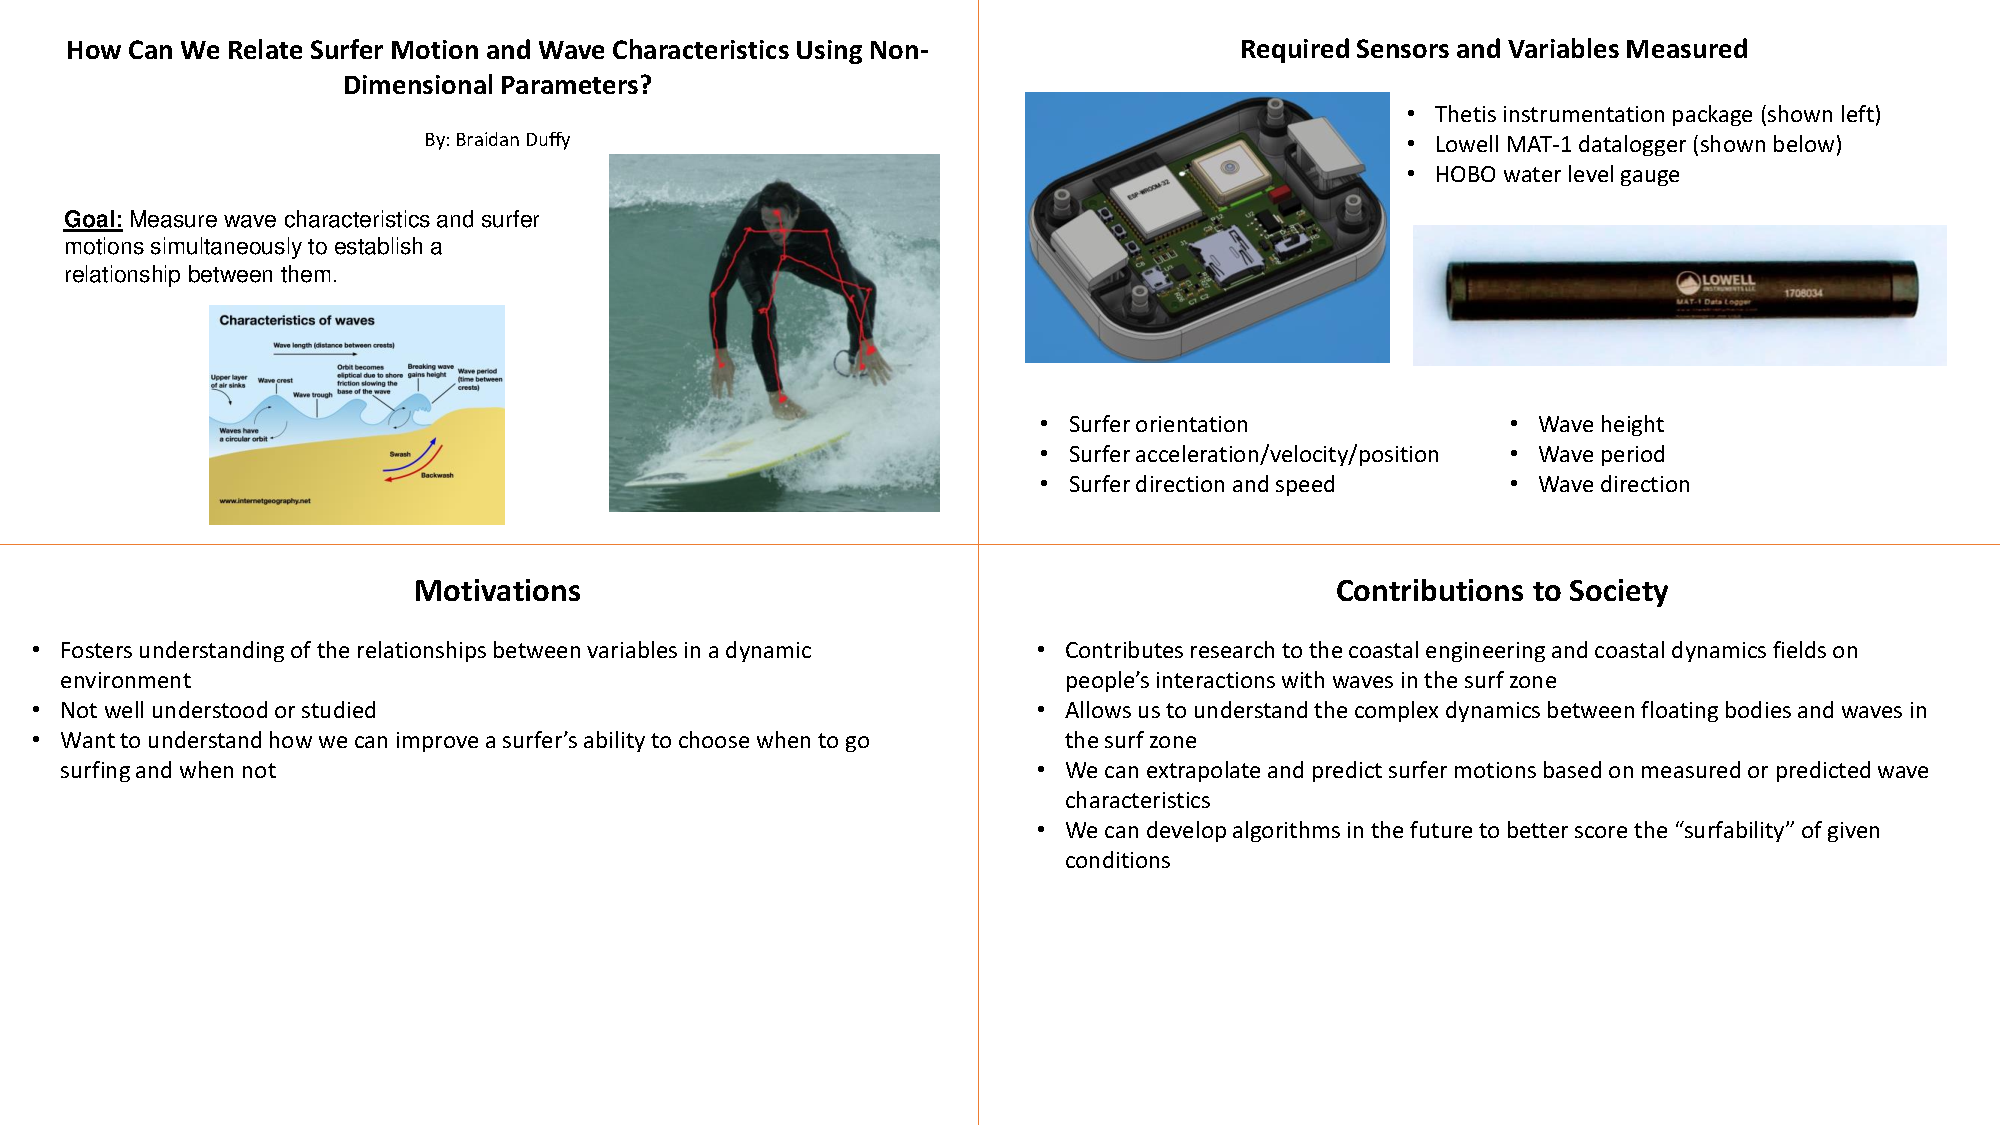
\includepdf[landscape=true]{../../publish/h2_quad_chart_example.pdf}

\end{document}